% The local minimal TeX image may lack ACM's scalable Libertine fonts.
% Disable font expansion only for that fallback so standard builds still work.
\IfFileExists{libertine.sty}{}{%
  \PassOptionsToPackage{expansion=false}{microtype}%
}
\documentclass[sigconf]{acmart}

\usepackage{amsmath}
\usepackage{booktabs}
\usepackage{tabularx}
\usepackage{array}
\usepackage{multirow}
\usepackage{xspace}
\usepackage{xcolor}
\usepackage{tikz}
\usepackage{balance}
\usetikzlibrary{arrows.meta,positioning,fit,calc}

\setcopyright{none}
\settopmatter{printacmref=true}
\renewcommand\footnotetextcopyrightpermission[1]{}
\acmConference[SIGMOD '27 Industrial Track]{2027 ACM SIGMOD/PODS Conference, Industrial Track}{June 13--18, 2027}{Huntington Beach, CA, USA}
\acmYear{2027}

\newcommand{\forlzero}{ForL0\xspace}
\newcommand{\system}{\forlzero}
\newcolumntype{L}[1]{>{\raggedright\arraybackslash}p{#1}}
\newcolumntype{C}[1]{>{\centering\arraybackslash}p{#1}}
\newcolumntype{Y}{>{\raggedright\arraybackslash}X}
\setlength{\emergencystretch}{1.5em}

\begin{document}

\title{\forlzero: A Cache-Aware Native State Backend for Apache Flink}

% SIGMOD Industrial Track is non-anonymous and requires at least one
% non-academic author. Replace this placeholder before submission.
\author{Author list pending}
\affiliation{%
  \institution{Huazhong University of Science and Technology and industrial collaborator}%
  \city{Wuhan}%
  \country{China}%
}

\begin{abstract}
Stateful stream processing increasingly runs with large in-memory working sets, where object-heavy heap layouts, pointer chasing, and garbage collection become first-order costs. We present \system, a production-oriented keyed-state backend for Apache Flink that retains the State API and checkpoint semantics while moving the authoritative state into a compact native engine. \system combines key-group and namespace-aware routing, Swiss-table-style group probing, typed JNI paths, an optional set-associative hot-key cache backed by the user-managed L0 partition on Kunpeng processors, and copy-on-write snapshots. It supports ValueState, ListState, MapState, ReducingState, and AggregatingState without application changes.

We evaluate \system on Intel x86\_64 and Kunpeng aarch64 servers. All 184 Java and native tests pass, including checkpoint, savepoint, restore, rescale, and mixed-state cases. On Intel, \system improves all 36 WordCount configurations by 1.270$\times$ on average and 1.414$\times$ at peak; VTune attributes the gain to a reduction in Memory Bound from 48.1\% to 15.3\%. On NexMark, \system retains a 1.39$\times$ geometric-mean speedup even with a normal 20~GB TaskManager budget. Under tight memory, it prevents Full-GC collapse and accelerates Kunpeng q4, q19, and q20 by 4.87$\times$, 5.36$\times$, and 5.96$\times$. These results show that compact state layout and off-heap ownership improve both steady-state efficiency and operational stability, while the L0 cache provides a smaller, workload-dependent increment.
\end{abstract}

\ccsdesc[500]{Information systems~Stream management}
\ccsdesc[300]{Information systems~Data structures}
\ccsdesc[300]{Computer systems organization~Heterogeneous (hybrid) systems}

\keywords{stream processing, Apache Flink, state backend, memory locality, native storage, checkpointing}

\maketitle

\section{Introduction}

Stateful stream processors maintain continuously changing per-key state for aggregation, joins, windows, timers, and online feature computation. Apache Flink exposes this state through a uniform API and couples it with consistent checkpointing and key-group-based redistribution \cite{carbone2015flink,carbone2017statemanagement}. The abstraction is operationally valuable, but it hides a physical question that becomes decisive at scale: how many objects, pointers, cache lines, and heap-management actions are required for one logical state access?

Flink's heap backend provides a short software path when state is small, but large object graphs increase pointer chasing and garbage-collection pressure. RocksDB bounds JVM heap use, yet introduces serialization, compaction, and storage-engine overhead \cite{rocksdb}. This leaves a useful middle ground for latency-sensitive workloads whose state should remain memory-resident: retain Flink's API and fault-tolerance contract, but organize the state as a compact native data structure.

\begingroup
\color{red}
\paragraph{Motivation study.}
Figure~\ref{fig:motivation-schematic} summarizes a controlled ValueState read--modify--write study after the state footprint reaches steady state. With ample heap headroom, per-operation access cost remains low while the active working set fits in the last-level cache (LLC), but increases by \textbf{TBD} once the working set outgrows the LLC, together with higher LLC-miss and memory-stall rates. Independently, at a fixed state footprint, GC time and pause cost rise sharply after the post-GC live heap exceeds \textbf{TBD}\% of \texttt{-Xmx}. These results expose a two-stage scalability problem: locality loss penalizes state access before memory exhaustion, and insufficient allocation headroom then turns heap-resident state into an operational-stability risk. This motivates a state backend that reduces both state-access overhead and JVM garbage-collection pressure. The current red curves and values are placeholders pending repeated-run measurements.
\endgroup

\begin{figure*}[t]
\centering
\color{red}
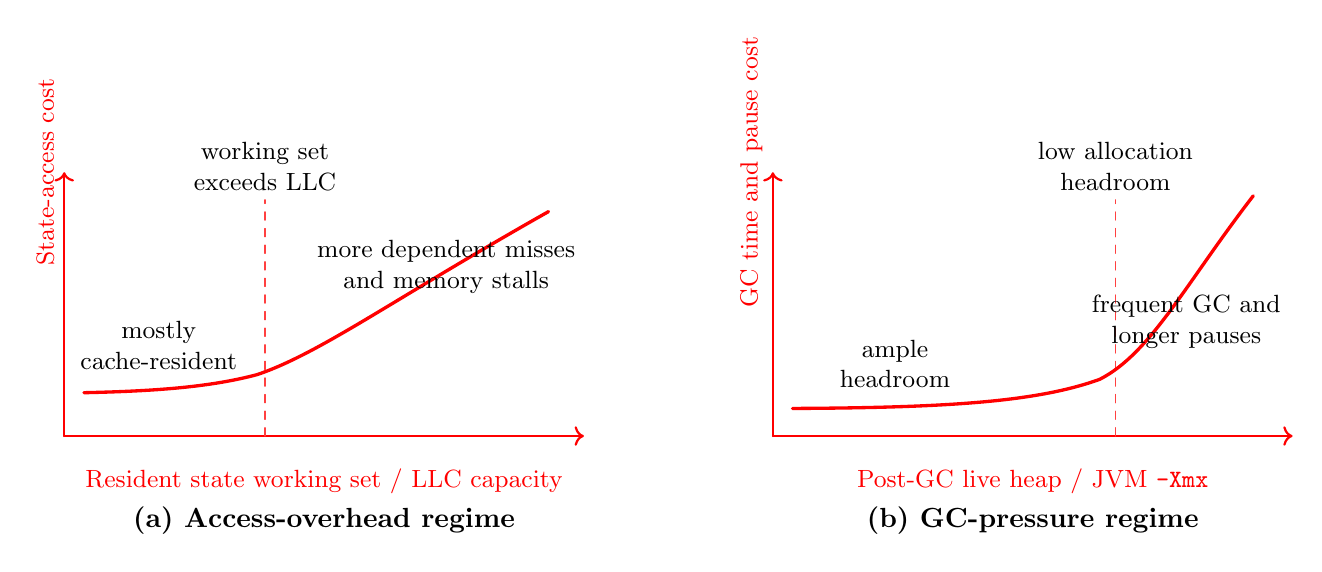
\begin{tikzpicture}[font=\small, line cap=round, line join=round]
  % Panel (a): state-access cost as the working set outgrows LLC.
  \begin{scope}[xshift=0cm]
    \draw[->, thick, red] (0,0) -- (6.6,0)
      node[below=8pt, midway, align=center] {Resident state working set / LLC capacity};
    \draw[->, thick, red] (0,0) -- (0,3.35)
      node[above, rotate=90, anchor=south] {State-access cost};
    \draw[dashed, red!75] (2.55,0) -- (2.55,3.0);
    \node[above, align=center] at (2.55,3.0) {working set\\exceeds LLC};
    \draw[very thick, red]
      (0.25,0.55) .. controls (1.15,0.57) and (1.85,0.62) .. (2.45,0.78)
      .. controls (3.25,1.05) and (4.2,1.75) .. (6.15,2.85);
    \node[align=center] at (1.2,1.15) {mostly\\cache-resident};
    \node[align=center] at (4.85,2.15) {more dependent misses\\and memory stalls};
    \node[font=\bfseries] at (3.3,-1.08) {(a) Access-overhead regime};
  \end{scope}

  % Panel (b): GC cost as the live heap approaches the JVM limit.
  \begin{scope}[xshift=9.0cm]
    \draw[->, thick, red] (0,0) -- (6.6,0)
      node[below=8pt, midway, align=center] {Post-GC live heap / JVM \texttt{-Xmx}};
    \draw[->, thick, red] (0,0) -- (0,3.35)
      node[above, rotate=90, anchor=south] {GC time and pause cost};
    \draw[dashed, red!75] (4.35,0) -- (4.35,3.0);
    \node[above, align=center] at (4.35,3.0) {low allocation\\headroom};
    \draw[very thick, red]
      (0.25,0.35) .. controls (2.2,0.36) and (3.35,0.43) .. (4.15,0.72)
      .. controls (4.8,1.05) and (5.25,1.95) .. (6.1,3.05);
    \node[align=center] at (1.55,0.92) {ample\\headroom};
    \node[align=center] at (5.25,1.45) {frequent GC and\\longer pauses};
    \node[font=\bfseries] at (3.3,-1.08) {(b) GC-pressure regime};
  \end{scope}
\end{tikzpicture}
\caption{\textcolor{red}{Motivation study. (a) State-access cost as the active working set outgrows the LLC. (b) GC time and pause cost as the post-GC live heap approaches the JVM heap limit. Together, the two regimes motivate reducing both state-access overhead and JVM garbage-collection pressure. Curves are placeholders pending measured data.}}
\Description{Two red schematic plots. State-access cost rises after the state working set exceeds the last-level cache, and garbage-collection cost rises sharply when the live heap approaches the JVM heap limit.}
\label{fig:motivation-schematic}
\end{figure*}

This design problem arose in a joint effort to accelerate Flink Heap State on heterogeneous processors, with a particular interest in Kunpeng's user-managed L0 cache partition. Early prototypes showed that placing a small cache above an object-heavy heap table was insufficient: the main table, JNI boundary, type conversions, and snapshot path still determined most costs. The resulting system, \system, therefore treats hardware caching as one component of a complete state backend rather than as an isolated optimization.

\system has three complementary mechanisms. First, it stores authoritative keyed state in native, cache-conscious Swiss-table-style structures partitioned by Flink key-group and namespace. Second, it selects typed JNI paths at state initialization, avoiding repeated type dispatch and eliminating serialization for common primitive and RowData layouts. Third, it takes asynchronous checkpoints from a copy-on-write view, allowing online updates to continue while preserving the checkpoint boundary. On Kunpeng, a set-associative L0 hot-key cache precedes the main table and transparently falls back on a miss.

This paper makes four contributions:
\begin{itemize}
  \item We describe a complete Flink 1.20.3 keyed-state backend spanning Java API compatibility, typed JNI, a native state engine, checkpoint/restore, and transparent deployment through Flink's SPI.
  \item We present a locality-oriented state layout and an 8-way L0 hot-key cache whose tags, keys, and values occupy three aligned cache lines per set.
  \item We show how copy-on-write overlays preserve Flink checkpoint, savepoint, and rescale semantics without maintaining a duplicate Java state table.
  \item We report a two-platform evaluation covering 184 correctness tests, 36-point WordCount grids, 14 state operations, eight NexMark queries, three memory budgets, an L0 ablation, and VTune microarchitectural evidence.
\end{itemize}

The central empirical result is not limited to memory exhaustion. Under a normal 20~GB TaskManager budget, \system still reduces the aggregate runtime of eight NexMark queries from 509~s to 343~s and achieves a 1.39$\times$ geometric-mean speedup. Tight memory amplifies the benefit by exposing the instability of heap-resident state, but it is not the only condition under which the backend helps.

\section{Context and Requirements}

\subsection{Flink Keyed State}

Flink partitions keyed state into key-groups. Each state descriptor supplies key, namespace, and value serializers, while the backend implements the physical representation and participates in checkpoint, savepoint, restore, and rescale. Operators may use a void namespace, as in simple per-key aggregates, or many namespaces, as in windowed workloads. A replacement backend must preserve these semantics across ValueState, ListState, MapState, ReducingState, and AggregatingState.

The backend must also coexist with Flink-managed priority queues and timers. \system deliberately reuses Flink's priority-queue implementation and replaces only the primary keyed-state data plane. This limits semantic risk and isolates the part of the runtime where memory layout is most important.

\subsection{Why the Heap Path Becomes Expensive}

Heap-resident state compounds three costs. First, hash metadata, boxed keys, namespaces, and values are separate objects, so one lookup may require several dependent cache misses. Second, a large live object graph increases tracing and evacuation work for the JVM. Third, generic serializers and state wrappers repeat type checks on the per-record path. These costs interact: under generous memory, they reduce throughput; under tight memory, they can trigger repeated Full GC and turn a slow query into an operational failure.

Our design requirements are therefore: (1) preserve Flink semantics and deployment compatibility; (2) reduce pointer chasing and heap residency; (3) specialize common layouts without losing a generic fallback; (4) keep checkpoint preparation short and serialization asynchronous; and (5) exploit Kunpeng L0 when present without making correctness depend on it.

\section{System Architecture}

Figure~\ref{fig:architecture} shows the four-layer organization. The Java control layer implements Flink interfaces, tracks the current key and key-group, validates serializers, registers state, and precomputes access strategies. Typed JNI functions carry compact arguments into the native engine. The native engine owns StateTables, namespace routing, Swiss tables, hot-key caches, and copy-on-write metadata. It is the single source of truth for keyed state; Java does not maintain a shadow copy.

\begin{figure*}[t]
\centering
\resizebox{0.92\textwidth}{!}{%
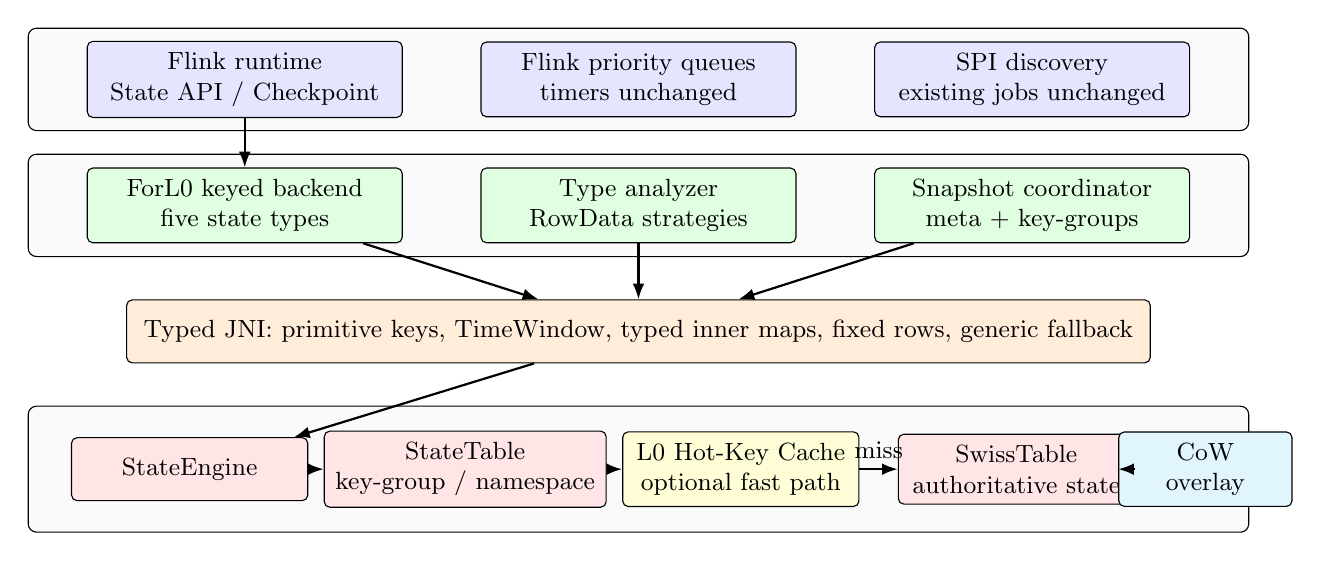
\begin{tikzpicture}[
  font=\small,
  box/.style={draw, rounded corners=2pt, align=center, minimum height=0.8cm, inner sep=4pt},
  lane/.style={draw, rounded corners=3pt, fill=black!2, minimum height=1.3cm},
  arr/.style={-{Latex[length=2mm]}, thick}
]
  \node[lane, minimum width=15.5cm] at (8,6.2) {};
  \node[box, fill=blue!10, minimum width=4.0cm] (api) at (3.0,6.2) {Flink runtime\\State API / Checkpoint};
  \node[box, fill=blue!10, minimum width=4.0cm] (pq) at (8.0,6.2) {Flink priority queues\\timers unchanged};
  \node[box, fill=blue!10, minimum width=4.0cm] (spi) at (13.0,6.2) {SPI discovery\\existing jobs unchanged};
  \node[lane, minimum width=15.5cm] at (8,4.6) {};
  \node[box, fill=green!12, minimum width=4.0cm] (backend) at (3.0,4.6) {ForL0 keyed backend\\five state types};
  \node[box, fill=green!12, minimum width=4.0cm] (types) at (8.0,4.6) {Type analyzer\\RowData strategies};
  \node[box, fill=green!12, minimum width=4.0cm] (snap) at (13.0,4.6) {Snapshot coordinator\\meta + key-groups};
  \node[box, fill=orange!15, minimum width=13.0cm] (jni) at (8.0,3.0) {Typed JNI: primitive keys, TimeWindow, typed inner maps, fixed rows, generic fallback};
  \node[lane, minimum width=15.5cm, minimum height=1.6cm] at (8,1.25) {};
  \node[box, fill=red!10, minimum width=3.0cm] (engine) at (2.3,1.25) {StateEngine};
  \node[box, fill=red!10, minimum width=3.0cm] (table) at (5.8,1.25) {StateTable\\key-group / namespace};
  \node[box, fill=yellow!16, minimum width=3.0cm] (hot) at (9.3,1.25) {L0 Hot-Key Cache\\optional fast path};
  \node[box, fill=red!10, minimum width=3.0cm] (swiss) at (12.8,1.25) {SwissTable\\authoritative state};
  \node[box, fill=cyan!12, minimum width=2.2cm] (cow) at (15.2,1.25) {CoW\\overlay};
  \draw[arr] (api) -- (backend);
  \draw[arr] (types) -- (jni);
  \draw[arr] (backend) -- (jni);
  \draw[arr] (snap) -- (jni);
  \draw[arr] (jni) -- (engine);
  \draw[arr] (engine) -- (table);
  \draw[arr] (table) -- (hot);
  \draw[arr] (hot) -- node[above]{miss} (swiss);
  \draw[arr] (swiss) -- (cow);
\end{tikzpicture}%
}
\caption{\system architecture. Flink-facing control remains in Java; the authoritative keyed-state data plane, optional L0 cache, and snapshot overlay reside in the native engine.}
\Description{A four-layer architecture showing Flink runtime services, the Java backend and type analyzer, typed JNI, and the native StateEngine, StateTable, hot-key cache, SwissTable, and copy-on-write overlay.}
\label{fig:architecture}
\end{figure*}

\subsection{State Registration and Access Strategies}

When a state descriptor is first used, the Java layer validates serializer compatibility and maps it to a native type layout. Supported primitive layouts include 32- and 64-bit integers, floating-point values, and booleans; structured layouts include strings, byte arrays, lists, maps, fixed rows, void namespaces, and TimeWindow namespaces. The backend then selects a ValueState, ListState, or MapState strategy once. Subsequent accesses enter a narrow JNI function instead of repeating serializer inspection.

RowData keys use three paths: a single primitive field is unboxed directly, fixed-length multi-field rows map to a compact native FixedRow, and variable-length rows use a generic byte representation. Selected BinaryRowData values can be returned through a read-only native memory view, avoiding an intermediate byte-array copy. Unsupported combinations retain a serializer-mediated fallback, so specialization does not narrow the State API.

\subsection{State Ownership and Namespace Routing}

Each task owns one StateEngine. A registered descriptor maps to one typed StateTable, and the table is partitioned first by key-group and then by namespace:
\begin{equation}
S: \mathrm{keyGroup} \rightarrow \mathrm{namespace} \rightarrow \mathrm{SwissTable}\langle K,V\rangle.
\end{equation}
For a void namespace, a key-group points directly to its SwissTable and avoids a namespace lookup. General namespaces use a map from namespace to independent sub-tables; empty namespace tables are removed eagerly. This layout aligns storage, checkpoint iteration, and rescale granularity.

Table~\ref{tab:state-paths} makes the per-state mapping explicit. The design does not encode a Java object graph in native memory. Instead, the outer keyed-state lookup and, where applicable, the inner container use independently typed layouts. ReducingState and AggregatingState deliberately keep user-code execution in Java: only the durable accumulator crosses into the native data plane.

\begin{table*}[t]
\caption{State API to native representation and execution path. ``Typed'' means that serializer inspection is performed at registration rather than on every access.}
\label{tab:state-paths}
\centering
\small
\begin{tabularx}{\textwidth}{L{2.2cm}L{3.2cm}L{4.1cm}Y}
\toprule
Flink state & Native value & Common operation path & Compatibility / fallback \\
\midrule
ValueState & Scalar, bytes, string, or fixed row & Typed point lookup; primitive return or read-only BinaryRowData view when eligible & Generic serializer path for variable layouts \\
ListState & Native element vector & Append/update in native container; batch iterator amortizes JNI on reads & Serializer-mediated element path; namespace merge preserves Flink order \\
MapState & Typed inner hash map & Outer key routes once; inner get/put/remove/contains avoids materializing the full Java map & Opaque serialized map for unsupported key/value combinations \\
ReducingState & Reduced value & Read accumulator, execute \texttt{ReduceFunction} in Java, write typed result & User function and null semantics remain unchanged \\
AggregatingState & Accumulator & Native accumulator storage; create/add/merge/result executed by the Flink function & Result materialization follows the registered serializer \\
\bottomrule
\end{tabularx}
\end{table*}

\section{Cache-Aware State Access}

\subsection{Swiss-Table Main Store}

The authoritative table stores one control byte per slot in a contiguous control array and key/value payloads inline. A hash is split into $H_1$, which selects the first probe group, and a seven-bit $H_2$ fingerprint stored in the control byte:
\begin{equation}
H_1=h\gg 7, \qquad H_2=h\;\&\;0x7F.
\end{equation}
A probe loads a group of control bytes, compares all fingerprints with SWAR or architecture-specific SIMD, and dereferences only matching payload slots. Empty and deleted markers support early termination and tombstones. Capacity is a power of two; growth performs a rehash into a larger table. Unlike a separate index/value-store design, the selected key and value are colocated in the slot, avoiding an additional value-pointer traversal.

\begin{figure}[t]
\centering
\resizebox{\columnwidth}{!}{%
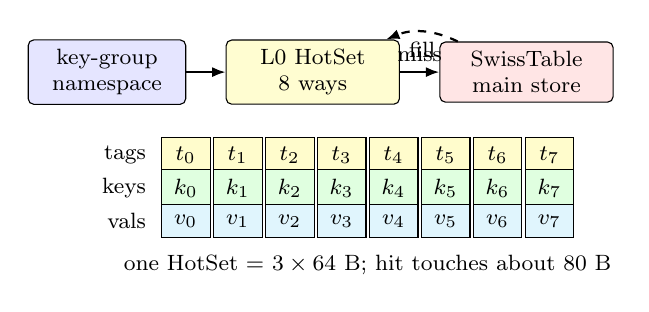
\begin{tikzpicture}[
 font=\footnotesize,
 cell/.style={draw, minimum width=0.62cm, minimum height=0.42cm, align=center},
 box/.style={draw, rounded corners=2pt, align=center, minimum height=0.65cm},
 arr/.style={-{Latex[length=1.7mm]}, thick}
]
 \node[box, fill=blue!10, minimum width=2.0cm] (route) {key-group\\namespace};
 \node[box, fill=yellow!18, minimum width=2.2cm, right=0.5cm of route] (cache) {L0 HotSet\\8 ways};
 \node[box, fill=red!10, minimum width=2.2cm, right=0.5cm of cache] (main) {SwissTable\\main store};
 \draw[arr] (route) -- (cache);
 \draw[arr] (cache) -- node[above]{miss} (main);
 \draw[arr, dashed] (main) to[bend right=24] node[below]{fill} (cache);
 \foreach \i in {0,...,7} {
   \pgfmathsetmacro{\xx}{1.0+0.66*\i}
   \node[cell, fill=yellow!20] at (\xx,-1.05) {$t_{\i}$};
   \node[cell, fill=green!12] at (\xx,-1.47) {$k_{\i}$};
   \node[cell, fill=cyan!12] at (\xx,-1.89) {$v_{\i}$};
 }
 \node[anchor=east] at (0.62,-1.05) {tags};
 \node[anchor=east] at (0.62,-1.47) {keys};
 \node[anchor=east] at (0.62,-1.89) {vals};
 \node at (3.31,-2.45) {one HotSet = $3\times64$ B; hit touches about 80 B};
\end{tikzpicture}%
}
\caption{Two-level lookup and the 8-way L0 HotSet. Tags, keys, and values occupy three aligned 64-byte rows; a miss falls back to the authoritative SwissTable.}
\Description{A two-level state lookup with an optional L0 cache before the SwissTable, plus an eight-way HotSet organized as tag, key, and value rows.}
\label{fig:hotpath}
\end{figure}

\subsection{Kunpeng L0 Hot-Key Cache}

On supported Kunpeng systems, \system allocates an outer cache from the user-managed L0 partition. It is a set-associative hash table with $N$ sets and eight ways per set. Each aligned set occupies 192 bytes: one 64-byte tag row, one key row, and one value row. A mixed 64-bit hash supplies $H_2$ as the tag and $H_1\,\&\,(N-1)$ as the set index. NEON \texttt{vceq\_u8} compares all eight tags; a scalar path is used elsewhere. A hit reads the 64-byte tag row plus one 8-byte key and value, approximately 80 bytes total.

Updates are write-through: the SwissTable is updated first, then the cache entry is inserted or replaced. Empty ways are preferred; otherwise a three-bit round-robin pointer stored in the tag row selects a victim. Deletes invalidate the tag. The cache is never part of the checkpoint image and can be rebuilt after restore, which keeps it outside the correctness boundary. If the L0 device or runtime library is absent, allocation transparently falls back and the main table remains fully functional.

\subsection{Five State Types}

ValueState maps to point lookup, update, and removal. ListState stores a native list container and supports append, update, and iteration. MapState uses a typed inner map so that an outer Flink key routes to a native map without reconstructing a Java object graph. ReducingState and AggregatingState invoke the user function in Java but store the accumulated value through the same typed native path. The common StateTable substrate ensures that all five types share namespace isolation, key-group ownership, snapshots, and restore.

\section{Checkpoint, Restore, and Rescale}

Flink initiates a checkpoint on the task thread but writes state asynchronously. \system separates these phases. During synchronous preparation, the StateEngine marks every participating key-group as snapshot-active and creates an overlay. The online table remains writable. On the first update after the boundary, the overlay records the old value; a new key is marked as post-snapshot and excluded; a deletion records the deleted value. The asynchronous writer reconstructs the $t_0$ view by merging the current table with the overlay.

\begin{figure}[t]
\centering
\resizebox{\columnwidth}{!}{%
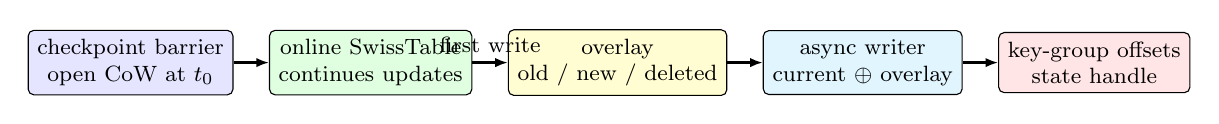
\begin{tikzpicture}[
 font=\footnotesize,
 box/.style={draw, rounded corners=2pt, align=center, minimum height=0.6cm, minimum width=2.3cm},
 arr/.style={-{Latex[length=1.6mm]}, thick}
]
 \node[box, fill=blue!10] (t0) {checkpoint barrier\\open CoW at $t_0$};
 \node[box, fill=green!12, right=0.45cm of t0] (online) {online SwissTable\\continues updates};
 \node[box, fill=yellow!18, right=0.45cm of online] (ov) {overlay\\old / new / deleted};
 \node[box, fill=cyan!12, right=0.45cm of ov] (writer) {async writer\\current $\oplus$ overlay};
 \node[box, fill=red!10, right=0.45cm of writer] (handle) {key-group offsets\\state handle};
 \draw[arr] (t0) -- (online);
 \draw[arr] (online) -- node[above]{first write} (ov);
 \draw[arr] (ov) -- (writer);
 \draw[arr] (writer) -- (handle);
\end{tikzpicture}%
}
\caption{Copy-on-write checkpoint path. The synchronous phase establishes the $t_0$ boundary; serialization proceeds asynchronously while the task continues processing.}
\Description{A checkpoint barrier opens copy-on-write, online updates populate an overlay, and an asynchronous writer combines the table and overlay into a keyed state handle.}
\label{fig:cow}
\end{figure}

The writer emits Flink's keyed-backend serialization metadata, priority-queue blocks, and native KV blocks with state identifiers and entry counts. Namespace, key, and value encodings follow their serializers. Restore validates the key serializer, recreates state metadata, restores priority queues, then rebuilds typed StateTables key-group by key-group. Canonical savepoints use the same builder with a translation step. Rescale redistributes key-groups; L0 sets are discarded and lazily repopulated.

The snapshot merge obeys three cases for every key first touched after $t_0$. An update records the pre-update value exactly once; an insertion records a post-snapshot marker; and a deletion retains the pre-delete value. During asynchronous enumeration, current entries marked as post-snapshot are skipped, current values with an overlay are replaced by the recorded old value, and deleted old values are emitted from the overlay. Therefore each key contributes exactly the value visible at $t_0$, independent of the number of subsequent writes.

\begin{table}[t]
\caption{Copy-on-write transition and asynchronous output rule.}
\label{tab:cow-rules}
\centering
\small
\begin{tabularx}{\columnwidth}{L{1.45cm}L{2.55cm}Y}
\toprule
First action after $t_0$ & Overlay record & Snapshot output \\
\midrule
Update & old value & old value replaces current value \\
Insert & post-$t_0$ marker & skip current entry \\
Delete & old value + deleted flag & emit old value from overlay \\
No change & none & emit current table value \\
\bottomrule
\end{tabularx}
\end{table}

Snapshot files are organized by key-group rather than by native allocation. Each key-group block carries the registered state identifier, entry count, namespace, key, and value bytes after serializer-compatible encoding. This is the unit Flink already assigns during rescale: restore reads only the handles intersecting the target key-group range and inserts entries into the newly constructed typed tables. The native memory address, SwissTable capacity, probe order, and hot-cache contents are intentionally absent from the durable format.

Resource lifetime is explicit. Successful and failed snapshots both release overlay state, restore failures destroy partially created engines, and backend disposal releases native tables and caches. This was essential in containerized deployments, where a leaked engine survives longer than an individual operator attempt.

\section{Implementation and Deployment}

\system targets Flink 1.20.3 and consists of a Java backend JAR plus a native shared library. The Java classes implement the standard backend factory and are discovered through SPI, so an existing job selects \system through configuration without changing application code. Native code uses C++17 and compiles on x86\_64 and aarch64. The Kunpeng build enables NEON matching and loads the L0 memory-pool library dynamically; L0 is a runtime option rather than a build-time dependency.

The JNI boundary carries engine and state handles, key-group identifiers, and typed payloads. One logical state operation performs one JNI transition in the common path. Batch and iterator interfaces amortize transitions for list and map traversal. The deployment bundle includes container images, offline dependencies, WordCount and NexMark harnesses, and build, usage, design, and test documents. This packaging matters for an industrial backend: reproducible installation and transparent fallback are as important as an isolated data-structure speedup.

\section{Evaluation}

We ask six questions: (Q1) Does \system preserve Flink state semantics? (Q2) Does the layout improve isolated state operations? (Q3) Does it improve a controlled per-record state workload? (Q4) Does it help end-to-end queries under normal memory? (Q5) Does off-heap state prevent collapse under tight memory? (Q6) What portion comes from L0 versus the main native layout?

\subsection{Platforms, Baselines, and Workloads}

Table~\ref{tab:setup} summarizes the environments. HashMapStateBackend is the direct in-memory baseline. WordCount performs a ValueState read-modify-write for two billion records at 36 combinations of 1--10 million keys and skew 0--1.0. The official Flink StateBackend JMH suite isolates ValueState, ListState, and MapState operations. NexMark uses q4, q5, q8, q9, q11, q18, q19, and q20, covering aggregation, windows, joins, lists, and maps \cite{tucker2008nexmark}.

\begin{table*}[t]
\caption{Experimental platforms and workload controls.}
\label{tab:setup}
\centering
\small
\begin{tabularx}{\textwidth}{L{2.1cm}L{4.2cm}Y}
\toprule
Item & Configuration & Purpose \tabularnewline
\midrule
Software & Flink 1.20.3; Java 8+; containerized standalone cluster; parallelism 8 & Same application logic and state API for both backends \tabularnewline
Intel x86\_64 & 1 JobManager + 2 TaskManagers; 4 cores/TM for the default run; 16/18/20~GB TM memory with 12/14/15~GB heap; no L0 hardware & WordCount, JMH, NexMark memory sweep, VTune \tabularnewline
Kunpeng aarch64 & openEuler; 4-core TM limit; 11.7~GB heap; 512~MB managed memory; L0 on/off & Tight-memory NexMark and L0 ablation \tabularnewline
WordCount & $2\times10^9$ records/run; keys $\in\{1,2,4,6,8,10\}$M; skew $\in\{0,.2,.4,.6,.8,1\}$; checkpoint off & Controlled steady-state state-access cost \tabularnewline
NexMark & q4, q5, q8, q9, q11, q18, q19, q20 & End-to-end stateful SQL/DataStream behavior \tabularnewline
\bottomrule
\end{tabularx}
\end{table*}

\begin{table*}[t]
\caption{NexMark query mix. Event counts differ by query so that each run reaches a stable, state-intensive phase while remaining operationally tractable.}
\label{tab:nexmark-workloads}
\centering
\small
\begin{tabular}{c r l@{\qquad}c r l}
\toprule
Query & Events & Stateful pattern & Query & Events & Stateful pattern \\
\midrule
q4  & 80M  & windowed category average & q5  & 80M  & sliding-window hot items \\
q8  & 100M & session window / new users & q9  & 40M  & two-stream winning-bid join \\
q11 & 80M  & per-user session window & q18 & 80M  & latest-result deduplication \\
q19 & 80M  & per-auction Top-10 & q20 & 60M  & grouped price aggregation \\
\bottomrule
\end{tabular}
\end{table*}

\paragraph{Measurement protocol.}
The WordCount grid contains $6\times6=36$ configurations and each backend processes exactly $2\times10^9$ records per configuration with checkpointing disabled. Throughput is the sink-observed total over parallelism eight. NexMark reports end-to-end completion time for the same query, event count, topology, and container limits under each backend. Ratios use $T_{heap}/T_{\system}$, so values above one favor \system; the cross-query summary is the geometric mean of per-query ratios rather than a ratio of unlike event totals. The available campaign records one completed run per configuration and therefore supports controlled case comparisons, not confidence intervals; repeated-run variance is a remaining measurement task.

\subsection{Q1: Correctness and Compatibility}

All 184 tests pass: 54 Java integration/unit tests and 130 native tests. Table~\ref{tab:correctness} shows the coverage rather than only the total. The campaign exercises all five state types, namespace semantics, periodic and externalized checkpoints, savepoints, asynchronous updates during a snapshot, restore, rescale, window aggregation, skew and stress, L0 fallback, and SPI discovery. Native tests cover SwissTable growth and tombstones, CoW round trips, serialization, TimeWindow namespaces, typed inner maps, and cache lifecycle.

\begin{table}[t]
\caption{Correctness coverage; all listed tests pass.}
\label{tab:correctness}
\centering
\small
\begin{tabularx}{\columnwidth}{L{2.7cm}C{1.0cm}Y}
\toprule
Layer & Tests & Representative coverage \tabularnewline
\midrule
Java / Flink & 54 & Five state types; checkpoint/savepoint; async snapshot; restore; rescale; windows; SPI \tabularnewline
Native engine & 130 & SwissTable; CoW; serialization round trip; namespaces; typed maps; HotCache \tabularnewline
\midrule
Total & 184 & 184 passed, 0 failed \tabularnewline
\bottomrule
\end{tabularx}
\end{table}

The result establishes semantic compatibility, not checkpoint-speed superiority. The current campaign validates completion and exact restored values; a matched checkpoint-duration and recovery-time study remains future work.

\subsection{Q2: Operator-Level State Cost}

On Intel, 13 of 14 JMH operations improve. The largest gains occur for list iteration (+131.5\%), map insertion (+110.0\%), value insertion (+87.2\%), map removal (+74.4\%), and value update (+59.5\%). List append regresses by 8.9\%, because a single append performs little probing work and exposes container/JNI overhead. The result is useful as a boundary: \system helps most when an operation performs lookup, iteration, or update work that benefits from compact layout; it is not uniformly faster for trivial calls.

\begin{table}[t]
\caption{Selected Intel StateBackend JMH changes over heap.}
\label{tab:jmh}
\centering
\small
\begin{tabular}{l r@{\qquad}l r}
\toprule
Operation & Change & Operation & Change \\
\midrule
value.Add & +87.2\% & value.Update & +59.5\% \\
map.Add & +110.0\% & map.Remove & +74.4\% \\
list.Iterate & +131.5\% & list.Append & $-$8.9\% \\
\bottomrule
\end{tabular}
\end{table}

\subsection{Q3: WordCount and Microarchitecture}

Table~\ref{tab:wordcount} reports representative points from the Intel grid. \system wins all 36 combinations, with a mean of 1.270$\times$ and a peak of 1.414$\times$. Each run processes two billion records; the mean wall-clock reduction is about 37~s. Intel has no L0 facility, so this result isolates the native layout, specialized access path, and group probing rather than the hardware cache.

\begin{table*}[t]
\caption{Representative Intel WordCount points (M records/s). All 36 scanned points favor \system.}
\label{tab:wordcount}
\centering
\small
\begin{tabular}{ccrrr@{\qquad}ccrrr}
\toprule
Keys & Skew & Heap & \system & Ratio & Keys & Skew & Heap & \system & Ratio \\
\midrule
1M & 0.0 & 13.153 & 17.464 & 1.328 & 2M & 0.0 & 12.140 & 17.170 & 1.414 \\
4M & 0.4 & 9.657 & 12.858 & 1.332 & 6M & 0.8 & 10.556 & 13.297 & 1.260 \\
8M & 1.0 & 11.162 & 15.028 & 1.346 & 10M & 0.2 & 9.933 & 12.476 & 1.256 \\
10M & 1.0 & 12.616 & 14.855 & 1.178 & \multicolumn{4}{r}{Mean over 36 points} & 1.270 \\
\bottomrule
\end{tabular}
\end{table*}

VTune explains the gain. Across matched 60.001~s collection windows, Memory Bound falls from 48.1\% to 15.3\%, DRAM Bound from 30.8\% to 2.2\%, and Back-End Bound from 58.1\% to 29.5\%. CPI decreases from 0.615 to 0.375, while Retiring rises from 30.4\% to 50.9\%. The reduction in memory stalls is therefore visible both in counters and application throughput.

Kunpeng WordCount is a contrasting result. Its 36-point mean ratio is 0.96$\times$, with ratios concentrated between 0.88 and 1.03. The workload performs only one read-modify-write per record and creates little GC pressure, so the fixed JNI cost offsets the native lookup benefit on this aarch64 system. This negative result prevents us from attributing all cross-platform gains to the hash table alone.

\subsection{Q4: NexMark under Normal Memory}

Table~\ref{tab:nexmark-normal} reports the Intel 20~GB setting, which provides a 15~GB heap and avoids the most severe memory pressure. \system still improves five of eight queries and matches heap on the other three. Across the eight queries, total runtime falls from 509~s to 343~s (32.6\%), and the geometric-mean speedup is 1.39$\times$. q19 and q20 improve by 2.86$\times$ and 2.21$\times$, while q4, q9, and q11 remain at parity. Thus, normal-memory NexMark already shows a material advantage; tight memory magnifies rather than creates it.

\begin{table}[t]
\caption{Intel NexMark with normal memory (20~GB TM / 15~GB heap), seconds.}
\label{tab:nexmark-normal}
\centering
\scriptsize
\setlength{\tabcolsep}{3pt}
\begin{tabular}{lrrrrrrrr}
\toprule
 & q4 & q5 & q8 & q9 & q11 & q18 & q19 & q20 \\
\midrule
Heap & 57 & 64 & 38 & 45 & 37 & 61 & 123 & 84 \\
\system & 57 & 52 & 36 & 45 & 37 & 35 & 43 & 38 \\
Ratio & 1.00 & 1.23 & 1.06 & 1.00 & 1.00 & 1.74 & 2.86 & 2.21 \\
\bottomrule
\end{tabular}
\end{table}

\subsection{Q5: Tight-Memory Stability}

On Kunpeng with 11.7~GB heap, 512~MB managed memory, and four TM cores, heap state repeatedly enters Full GC on q4, q9, q19, and q20. Table~\ref{tab:nexmark-tight} shows that \system completes every query. q4 drops from 716~s to 147~s (4.87$\times$), q19 from 638~s to 119~s (5.36$\times$), and q20 from 542~s to 91~s (5.96$\times$). q5 and q11 remain near parity, showing that gains follow state and memory pressure rather than a global runtime bias.

\begin{table}[t]
\caption{Kunpeng NexMark under tight memory, seconds. Stars mark heap runs heavily delayed by Full GC.}
\label{tab:nexmark-tight}
\centering
\scriptsize
\setlength{\tabcolsep}{2.1pt}
\resizebox{\columnwidth}{!}{%
\begin{tabular}{lrrrrrrrr}
\toprule
Backend & q4 & q5 & q8 & q9 & q11 & q18 & q19 & q20 \\
\midrule
Heap & 716$^\star$ & 103 & 72 & 201$^\star$ & 98 & 134 & 638$^\star$ & 542$^\star$ \\
\system with L0 & 147 & 103 & 62 & 105 & 96 & 93 & 119 & 91 \\
\system without L0 & 159 & 100 & 62 & 107 & 102 & 98 & 121 & 94 \\
\midrule
Heap / \system & 4.87 & 1.00 & 1.16 & 1.91 & 1.02 & 1.44 & 5.36 & 5.96 \\
\bottomrule
\end{tabular}
}
\end{table}

The Intel memory sweep exhibits the same transition. At 16~GB, heap q4 and q9 take 352~s and 232~s, while q19 and q20 fail to complete; \system finishes them in 61, 46, 47, and 40~s. At 18~GB, heap q19 and q20 still require 279 and 313~s versus 45 and 38~s. At 20~GB, the gap narrows but remains significant for q18--q20. Native ownership therefore converts a steep, GC-driven performance cliff into a comparatively flat response to the memory budget.

\begin{table*}[t]
\caption{Intel NexMark memory sweep, seconds. ``--'' denotes a heap run that did not complete because of repeated Full GC. H is JVM heap within the TaskManager budget.}
\label{tab:nexmark-sweep}
\centering
\small
\setlength{\tabcolsep}{4.0pt}
\begin{tabular}{llrrrrrrrr}
\toprule
TM / heap & Backend & q4 & q5 & q8 & q9 & q11 & q18 & q19 & q20 \\
\midrule
16G / H12G & Heap & 352 & 63 & 39 & 232 & 44 & 53 & -- & -- \\
             & \system & 61 & 56 & 36 & 46 & 35 & 34 & 47 & 40 \\
\midrule
18G / H14G & Heap & 156 & 64 & 36 & 46 & 53 & 53 & 279 & 313 \\
             & \system & 57 & 52 & 36 & 46 & 37 & 38 & 45 & 38 \\
\midrule
20G / H15G & Heap & 57 & 64 & 38 & 45 & 37 & 61 & 123 & 84 \\
             & \system & 57 & 52 & 36 & 45 & 37 & 35 & 43 & 38 \\
\bottomrule
\end{tabular}
\end{table*}

\subsection{Q6: L0 Contribution}

The Kunpeng ablation in Table~\ref{tab:nexmark-tight} shows a modest L0 increment over the native main table: q4 improves from 159~s to 147~s, q18 from 98~s to 93~s, and q20 from 94~s to 91~s; several queries are unchanged within a few seconds. NexMark performs substantial serialization, window management, and data exchange, so many records do not repeatedly hit a small value-state working set. The dominant end-to-end benefit is the native layout and removal of large state from the Java heap. L0 is most useful for fine-grained hot-key access and should be described as an accelerator, not as the sole cause of the system-level result.

\section{Industrial Lessons and Limitations}

\paragraph{A cache is not a backend.}
The initial goal emphasized Kunpeng L0, but experiments forced a broader design. Caching cannot repair pointer-heavy authoritative storage, repeated serialization, or a stop-the-world heap. The main contribution became an end-to-end native backend; L0 then added value on top of a sound data plane.

\paragraph{Normal and tight memory are different claims.}
Under normal memory, compact layout and typed paths improve state-heavy queries without relying on GC collapse. Under tight memory, moving state off heap additionally prevents Full GC and non-completion. Reporting only the largest tight-memory speedups would hide this distinction and overstate the role of one mechanism.

\paragraph{Fallbacks enabled deployment.}
The generic serializer path, scalar group match, and non-L0 allocator made the same plugin usable on Intel and Kunpeng. They also allowed correctness testing without special hardware. This widened the system's practical scope, although the fastest path still depends on recognizable primitive or fixed-row layouts.

\paragraph{Limitations.}
The two platforms are not intended as a normalized CPU comparison; they answer complementary questions under their own controlled baselines. The L0 ablation is end-to-end and does not include a dedicated hit-rate or cycle-level microbenchmark. Checkpoint and restore are validated for correctness, but matched duration and recovery-time numbers are not yet reported. The evaluation focuses on in-memory HashMapStateBackend rather than RocksDB/ForSt, and does not yet cover timer-dominated applications or long-running production traces. Finally, ListState append exposes JNI/container overhead and remains a target for batching.

\section{Related Work}

Flink, MillWheel, Naiad, the Dataflow model, and Structured Streaming establish the semantics and runtime models for consistent stateful stream processing \cite{carbone2015flink,akidau2013millwheel,murray2013naiad,akidau2015dataflow,armbrust2018structured}. Flink's state-management work focuses on checkpoint consistency and operational integration \cite{carbone2017statemanagement}, while Megaphone addresses low-disruption state migration \cite{hoffman2019megaphone}. \system preserves those semantic boundaries but focuses on the physical representation and access cost of local keyed state.

RocksDB provides a mature persistent backend with bounded heap use, compaction, and disk-aware behavior \cite{rocksdb}. \system targets a different point: memory-resident workloads that need low latency and predictable behavior without a Java object graph. FASTER demonstrates that carefully designed in-place updates and memory tiers can substantially change key-value performance \cite{chandramouli2018faster}. Swiss tables demonstrate the value of compact control metadata and group probing \cite{abseil2018swisstable}; \system adapts these ideas to Flink key-groups, namespaces, typed state containers, checkpoints, and an optional hardware-resident hot-key cache.

\section{Conclusion}

\system is a complete native keyed-state backend for Apache Flink, not merely a hash-table or cache prototype. It integrates five state types, typed JNI and RowData paths, cache-aware Swiss tables, an optional Kunpeng L0 hot-key cache, and copy-on-write checkpoint/restore behind the standard State API. All 184 correctness tests pass. The evaluation shows 1.270$\times$ mean WordCount throughput on Intel, reduced memory stalls, a 1.39$\times$ geometric-mean NexMark speedup under normal memory, and up to 5.96$\times$ under tight memory where heap state suffers Full GC. The results also establish a useful boundary: L0 adds a workload-dependent increment, while compact native state ownership provides the broad performance and stability benefit.

\balance
\bibliographystyle{ACM-Reference-Format}
\bibliography{briskstate_sigmod_industry}

\end{document}
